\documentclass{article}
\usepackage[utf8]{inputenc}

\title{Mek9250 - Mandatory Exercise}
\author{Florian Arbes}
\date{February 2021}

\usepackage{natbib}
\usepackage{minted}
\usepackage{graphicx}
\usepackage{subfig}
\usepackage{amsmath}
\begin{document}

\maketitle

\section*{Exercise 1}

The following equation is given on the domain $\Omega = (0, 1) ^2$:
\begin{align}
 - \mu \left( \frac{\partial^2 u}{\partial x^2} + \frac{\partial^2 u}{\partial y^2} \right)+ \frac{\partial u}{\partial x} &= 0 \quad in \quad  \Omega, \\
u &= 0 \quad for \quad x = 0 \\
u &= 1 \quad for \quad x = 1 \\
\frac{\partial u}{\partial n} &= 0 \quad for \quad y=0 \quad  and \quad y=1
\end{align}

\subsection*{a) An analytical solution}
Ansatz: $u(x, y) = u(x)$, which means $\frac{\partial u}{\partial y} = 0$ and  $\frac{\partial^2 u}{\partial y^2} = 0$. The PDE then simplifies to:

$$ \frac{\partial u}{\partial x} =  \mu \left( \frac{\partial^2 u}{\partial x^2} + 0 \right)$$
This ODE can be solved easily:

$$ \int_{\Omega} \frac{\partial u}{\partial x}  dx =  \mu  \int_{\Omega} \frac{\partial^2 u}{\partial x^2}  dx $$
$$ u = \mu  \frac{\partial u}{\partial x}  dx + C $$
Thus, $u(x)$ has the form $u(x) = A e^{Bx}+C$, with the derivatives $\frac{\partial u}{\partial x} = AB e^{Bx}$ and $\frac{\partial^2 u}{\partial x^2} = AB^2 e^{Bx}$. This can be plugged into the ODE:
$$AB e^{Bx} =\mu \left( AB^2 e^{Bx} +0 \right) \Leftrightarrow B = \frac{1}{\mu}$$
If $A$ and $C$ can be chosen in a way, that they fulfill the boundary conditions, $u(x)$ is a solution to the PDE as well.

\begin{align}
u &= 0  \quad for \quad x = 0  &\Rightarrow u(x=0) = A e^{0B} + C = 0\quad\quad\\
u &= 1  \quad for \quad x = 1 & \Rightarrow u(x=1) = A e^{1B} + C = 1\quad\quad\\
\frac{\partial u}{\partial n} &= 0 \quad for \quad y=0 \quad  and \quad y=1& \Rightarrow \frac{\partial u}{\partial y} = 0 \quad(for \quad all \quad y \quad true)
\end{align}
\\
Subtracting (5) from (6) leads to:
$$A e^{1B} - A = 1 \Leftrightarrow A = \frac {1}{e^B-1}$$
From (5) we get
$$C = -A = -\frac {1}{e^B-1}$$
\\
The solution therefore is:

$$u(x, y) = \frac {1}{e^B-1} e^{Bx}-\frac {1}{e^B-1} =(e^{Bx}-1) \frac {1}{e^B-1} = \frac {e^{\frac{x}{\mu}}-1}{e^\frac{1}{\mu}-1}$$

\subsection*{b) Numerical error for various h and various $\mu$}
Figure 1 shows the analytical and numerical solution for various mu (h = 1/8). As h decreased, the error decreases. The error can be estimated with
$$||u-u_h||_1 \leq C_{\alpha} h^{\alpha}$$
and
$$||u-u_h||_0 \leq C_{\beta} h^{\beta}$$
A curve fit is used to approximate $C_{\alpha}$, $\alpha$, $C_{\beta}$ and $\beta$ (see Figure 2). Since the scheme is $\mathcal{O}(h^2)$, $\alpha$ and $\beta$ should equal 2. The numerical approximations are listed in Table 1 for different values of $\mu$.

\begin{figure}
\centering
  \subfloat[mu = 1.0]{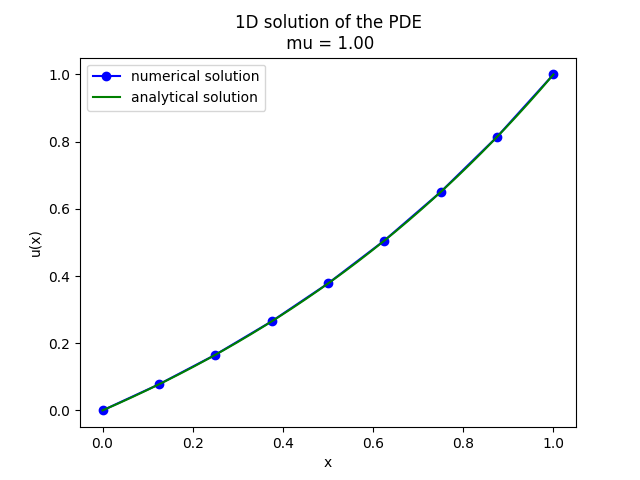
\includegraphics[width=0.5\textwidth]{mu1.png}\label{fig:f1}}
  \hfill
  \subfloat[mu = 0.01]{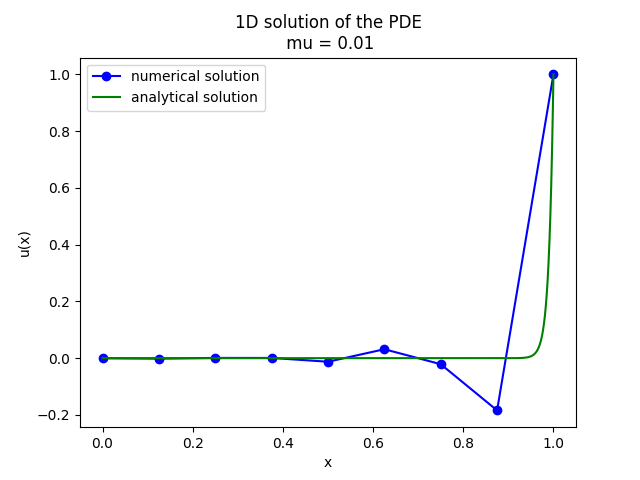
\includegraphics[width=0.5\textwidth]{mu001.png}\label{fig:f2}}
  \caption{Numerical solutions (h=1/8).}
\end{figure}

\begin{figure}
\centering
  \subfloat[mu = 1.0]{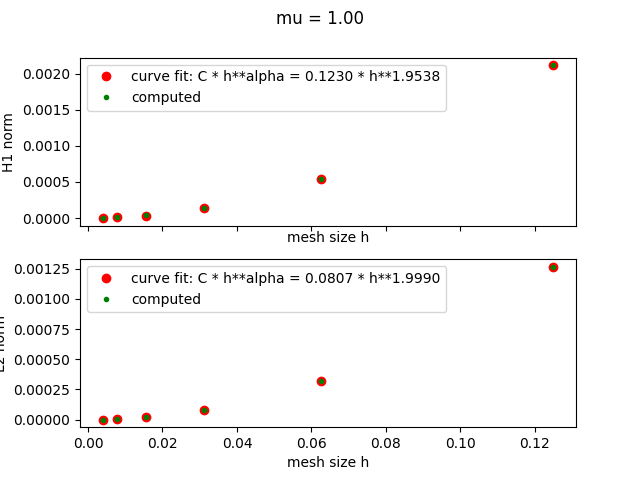
\includegraphics[width=0.5\textwidth]{curve1.png}\label{fig:f1}}
  \hfill
  \subfloat[mu = 0.01]{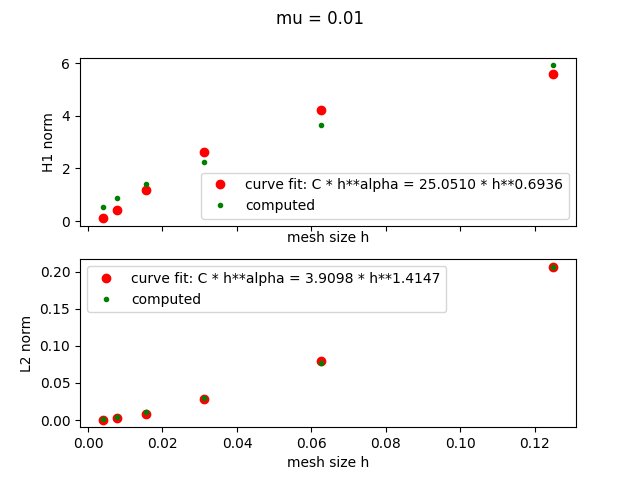
\includegraphics[width=0.5\textwidth]{curve01.png}\label{fig:f2}}
  \caption{curve fit for various h.}
\end{figure}





\begin{center}
 \begin{tabular}{||c c c c c||}
 \hline
mu & C_{alpha} & alpha & C_{beta} & beta \\ [0.5ex]
\hline\hline
1.00 & 0.1230 & 1.9538 & 0.0807 & 1.9990 \\
\hline
0.30 & 1.2157 & 1.8635 & 0.2559 & 1.9765 \\
\hline
0.10 & 8.3900 & 1.6440 & 0.9624 & 1.8894 \\
\hline
\end{tabular}
\end{center}

\subsection*{b) Numerical error with SUPG stabilization}
After introducing a stabilization, the numerical results look slightly different (see Figure 3). The error estimates are given in Table 2

\begin{figure}
\centering
  \subfloat[mu = 1.0]{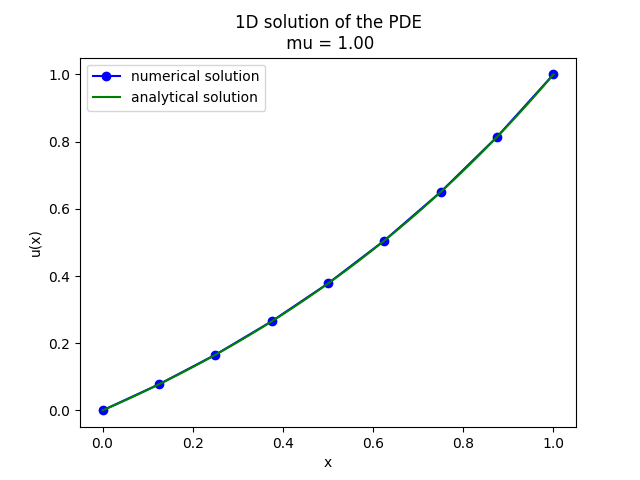
\includegraphics[width=0.5\textwidth]{mu1SUPG.png}\label{fig:f1}}
  \hfill
  \subfloat[mu = 0.01]{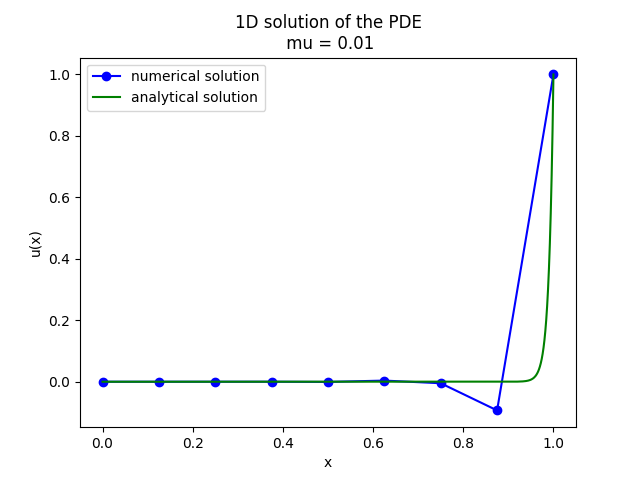
\includegraphics[width=0.5\textwidth]{mu001SUPG.png}\label{fig:f2}}
  \caption{Numerical solutions with SUPG stabilization (h=1/8).}
\end{figure}

\begin{center}
 \begin{tabular}{||c c c c c||}
 \hline
mu & C_{alpha} & alpha & C_{beta} & beta \\ [0.5ex]
\hline\hline
1.00 & 0.1220 & 1.9519 & 0.0845 & 2.0117 \\
\hline
0.30 & 0.9965 & 1.8073 & 0.3066 & 2.0286 \\
\hline
0.10 & 5.8300 & 1.5390 & 0.9880 & 1.8970 \\
\hline
\end{tabular}
\end{center}




\section*{Exercise 2}
The Navier-Stokes equations for incompressible fluids ($\nabla \cdot u = 0$) is defined as followed:
\begin{equation}
  \varrho \frac{ \partial  u}{\partial t} +  \varrho (u \cdot \nabla) u = \mu \nabla^2 u -\nabla \cdot pI + \varrho g
\end{equation}



The terms from left to right are the acceleration, convection, diffusion, pressure gradient and the body forces (such as gravity). The terms can be separated like that:
$$\varrho \frac{ \partial  u}{\partial t} = F(u, p) $$
The equations can be discretized in time, where $u^{n+1}$ denotes the time-step that needs to be computed. $u^{n}$ is then the known time-step. A fully explicit time discretization would be a forward euler scheme:
$$\varrho \frac{u^{n+1} - u^{n}}{\Delta t} = F(u^{n}, p^{n}) $$


\subsection*{a) Implement a solver for the benchmark problem.}
See code. It code can be executed from the command line like that:
\begin{minted}{python}
python chorin_proj_cylinder.py --d_velocity 2 --d_pressure 1 --explicit 1
\end{minted}



A semi-implicit discretization can be executed from the command line like that:
\begin{minted}{python}
python chorin_proj_cylinder.py --d_velocity 2 --d_pressure 1 --explicit 0
\end{minted}


\subsection*{b) Stability requirement}
The cfl number was found to be around 0.05 in order to have a stable scheme

\subsection*{c) Drag and lift}

The drag and lift coefficients were found to be $3.1846$ and $0.7358$ respectively, which is in the given bounds (see also Figure 4).


\begin{figure}[h]
    \centering
    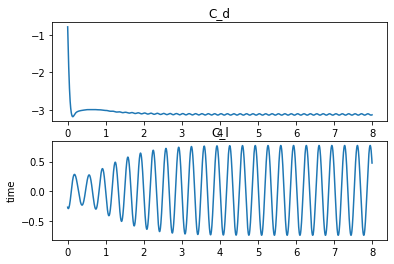
\includegraphics[width=0.75\textwidth]{draglift.png}
    \caption{Drag and lift coefficients}
    \label{fig:mesh1}
\end{figure}


\bibliographystyle{plain}
\bibliography{references}
\end{document}
